\section{Learning Paradigms}

\begin{frame}\frametitle{\secname}

\mode<article>{
There are three learning paradigms in machine learning:
}
\begin{itemize}
\item Supervised learning\notesonly{. Learning with a teacher (cf. \sectionref{sec:supervised}).}
\item Unsupervised learning\notesonly{. Learning only from observations, without a teacher (cf. \sectionref{sec:unsupervised}).}
\item Reinforcement learning\notesonly{. This is about maximizing reward (cf. \sectionref{sec:reinforcement}).}
\end{itemize}
\mode<article>{
It is possible to understand the differences between them by describing
\begin{inparaenum}[(i)]
    \item the data each of them deals with and
    \item the objective that each is trying to model
\end{inparaenum}
}
\mode<presentation>{

Differences: Data \& objective model.
}

\end{frame}


\subsection{Supervised learning} \label{sec:supervised}

\begin{frame}\frametitle{\subsecname}

\mode<article>Supervised learning is\mode<all>essentially function fitting.

\underline{Data}:\\
\mode<presentation>{\vspace{5mm}}

Consider this dataset of tuples:
\begin{equation}
\label{eq:tuples}
\left( \vec x^{(1)}, \vec y_T^{(1)} \right) \,,\, \ldots \,,\, \left( \vec x^{(\alpha)}, \vec y_T^{(\alpha)} \right) \,,\, \ldots \,,\, \left( \vec x^{(p)}, \vec y_T^{(p)} \right)
\end{equation}

\mode<article>{
where,
\begin{itemize}
\item[] $\vec x$ denotes the observation with $N$ components. $\vec x = (x_1, x_2, \ldots x_N)$, $\vec x \in \R^N$ (e.g. pixel values in an image)
\item[] $\vec y_T$ denotes the label assigned to this observation. It is also referred to as the ground truth.
When $y_T \in \R$ or $\vec y_T \in \R^M$, we are looking at a regression problem (e.g. predicting house prices, object localization - bounding box regression (x, y, w, h)).\\
When $y_T \in \{ 0, 1\}$, we refer to this as a binary classification problem (e.g. is this a cat or a dog).\\
When $y_T \in \{ 0, \ldots, K-1\}$, we refer to this as a multi-class classification problem (e.g. which letter is this?).
\item[] $p$ denotes the size of the dataset (i.e. how many labeled observations we have.)
\item[] The superscript $^{(\alpha)}$ denotes the index of a particular sample within the dataset. $\alpha = 1 , \ldots, p$
\item[] The samples are often assumed to be \emph{independent and identically distributed} (\iid).
\end{itemize}
}

%\end{frame}
\pause
%\begin{frame}

\underline{Objective model}:\\
\mode<presentation>{\vspace{5mm}}
\notesonly{Supervised learning algorithms are used to }find a function that maps observations to their label(s)\notesonly{ which represents some concept or value.
This mapping can be described in the form of:}
\begin{itemize}
\item a discrimination function $\vec y = \vec f(\vec x)$, \\ 

\notesonly{
where $\vec f(\cdot)$ denotes a vector valued function }$\vec f: \R^N \rightarrow \R^M$
\item a conditional distribution $P(\,\vec y \,|\, \vec x\,)$.
\end{itemize}

\end{frame}

\subsection{Unsupervised learning} \label{sec:unsupervised}

\begin{frame}\frametitle{\subsecname}

\mode<article>
Unsupervised learning tries to find 
\mode<all>
 interesting directions and/or structure in the data using only observations $\vec x \in \R^N$.

\underline{Data}:

A dataset of observations:
\begin{equation}
\label{eq:observations}
%\vec x^{(1)} \,,\, \ldots \,,\, \vec x^{(\alpha)} \,,\, \ldots \,,\, \vec x^{(p)}
\vec X = 
\left(
\begin{array}{cccccc}
\Big| & \Big| & & \Big| & & \Big| \\[3mm]
\vec x^{(1)} & \vec x^{(2)} & \cdots & \vec x^{(\alpha)} & \cdots & \vec x^{(p)}\\[2mm]
\Big| & \Big| & & \Big| & & \Big|
\end{array}
\right) \in \R^{N \times p}
\end{equation}
\notesonly{
where $p$ denotes the number of observations (i.e. size of the dataset) and $N$ denotes the number of dimensions.}
\slidesonly{
where 
\begin{itemize}
\item[] $p$ \corresponds\, no. of observations (often \iid)
\item[] $N$ \corresponds\, no. of dimensions
\end{itemize}
}
\notesonly{
The samples are often assumed to be \iid, but algorithms for handling sequential data also exist.

Example: $\vec x$ could represent user ratings, pixel values in images.
}
\end{frame}
\begin{frame}

\underline{Objective model}:
\mode<presentation>{\vspace{5mm}}
\mode<article>{
An unsupervised learning algorithm is used to capture structure or directions in the data. This can be achieved by finding:
}
\begin{itemize}
\item the underlying distribution $P(\vec x)$ that generated this data (e.g. density estimation),
\item $\vec z := \vec f(\vec x)$, where $\vec z$ is a measure of 
\begin{itemize}
\item possible structure such as clustering or grouping in the data ($\vec z \in {0,\ldots,K-1}$), \\

and/or

\item possible directions in the data, by finding another continuous space for describing this data. \\

Example: dimensionality reduction, $\vec z \in \R^M$ with $M < N$.

\end{itemize}
\end{itemize}

\end{frame}

\newpage

\subsection{Reinforcement learning} \label{sec:reinforcement}

\begin{frame}\frametitle{\subsecname}

Reinforcement learning is about what actions to take in which situations in order to maximize some reward.
This implies that learning happens through an interaction of the agent with its environment.

\end{frame}

\begin{frame}

\underline{Data}:

Our data consists of a sequence. Each time step is described by 

\begin{itemize}
\item a state $\vec x \in \mathcal{X}$ or $\vec x \in \R^N$, e.g. $\mathcal{X} := \{ \vec x_1, \ldots, \vec x_S\} \subset \{0,1\}^S$ (1-out-$S$ encoding)
\pause
\item an action $\vec a$ which can be taken by the agent:\\

$\vec a \in \mathcal{A}$ or $\vec a \in \R^M$, e.g. $\mathcal{A} := \{ \vec a_1, \ldots, \vec a_A\} \subset \{0,1\}^A$ (1-out-$A$ encoding)
\pause
\item a reward $r \in \R$ or $r \in \{0,1\}$, e.g. $r \in \{\text{``cheese''},\text{``no cheese''}\}$.

\end{itemize}
\pause
\mode<article>{Each time step describes what reward was received when performing some action while in some state. 
The sequence we observe becomes:}

\begin{align}
\label{eq:chain}
\left\{\vec x^{(t)}, \vec a^{(t)}, r^{(t)}\right\}_{t=0}^{p} = 
\left( \vec x^{(0)}, \vec a^{(0)}, r^{(0)} \right) \,,\, \ldots \,,\, \left(\vec x^{(p)}, \vec a^{(p)}, r^{(p)} \right)
\end{align}

\question{Can we still assume \iid?}

\mode<article>{
-Since we observe sequential data, we no longer assume \iid~\emph{within} a sequence. But if we have multiple sequences, we can assume \iid~\emph{across} sequences.
}

\end{frame}

\begin{frame}

Example:
\begin{itemize}
\item $\vec x \; \corresponds$ position in a maze
\item $\vec a \; \corresponds$ movement direction (velocity), e.g. turn left/right
\item $r \; \corresponds$ found the cheese, found smaller piece of cheese. A negative reward, ``punishment'' is also possible.
\end{itemize}
\end{frame}


\begin{frame}
    \mode<presentation>{
    \begin{figure}[h]
        \centering
        \only<1>{
        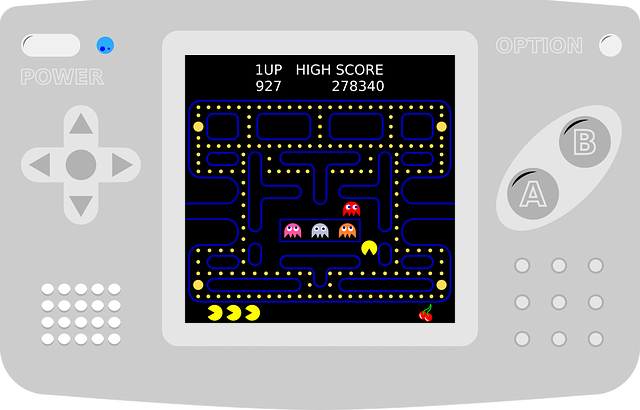
\includegraphics[height=5cm]{img/handheld-game-console-2134571_640}
        }
        \only<2>{
        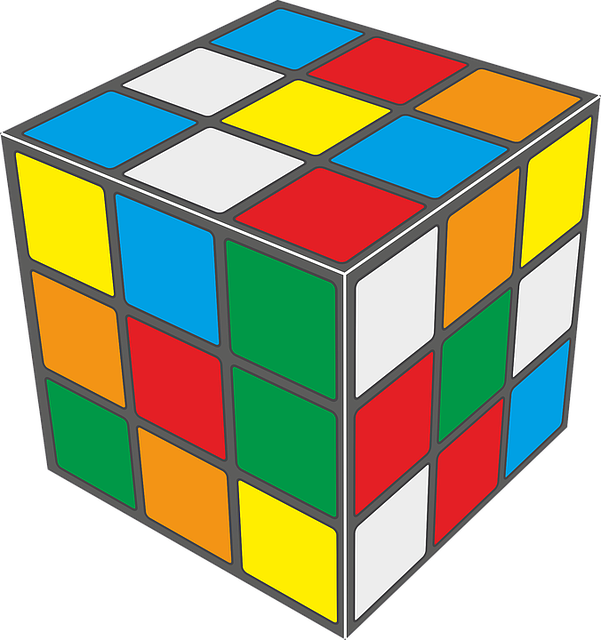
\includegraphics[height=3cm]{img/babyrajeshraj-1087832_640}
        }
    \end{figure}
    }
    
\question{What would be a state/action/reward here?}

\end{frame}

\mode<article>{
\begin{figure}[ht]
     \centering
     \savebox{\imagebox}{
	 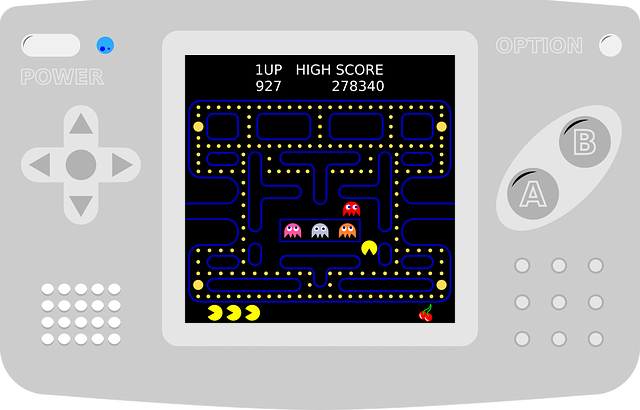
\includegraphics[width=0.2\textwidth]{img/handheld-game-console-2134571_640}}%
     \begin{subfigure}[t]{0.35\textwidth}
         \centering
         \usebox{\imagebox}% Place largest image
     \end{subfigure}
     \hspace{1mm}
     \begin{subfigure}[t]{0.25\textwidth}
         \centering
         \raisebox{\dimexpr.5\ht\imagebox-.5\height}{% Raise smaller image into place
         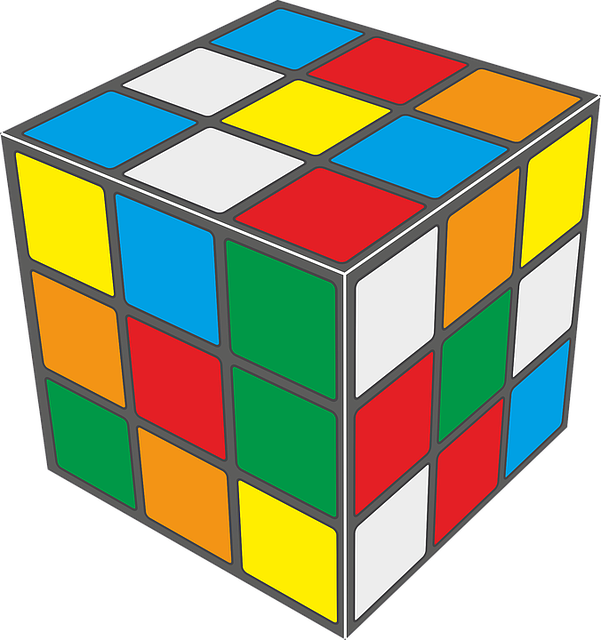
\includegraphics[width=0.5\textwidth]{img/babyrajeshraj-1087832_640}
         }
     \end{subfigure}
     \caption{Representing games for reinforcement learning}
\end{figure}
}

\begin{frame}

\underline{Objective model}:\\
\mode<presentation>{\vspace{5mm}}
Reinforcement learning can be used to:
\begin{itemize}
\item select the optimal action when arriving at a state: $\vec a^* = \vec f(\vec x, r)$
\item find the transition model $P(\vec x^{(t)}\,|\,\vec x{(t-1)}, \vec a^{(t-1)})$, where $t$ is a time step within the sequence.
\end{itemize}
\pause
\question{Would you regard reinforcement learning as supervised or unsupervised learning?}

\end{frame}

\newpage

\subsection{Summarized overview}

\begin{frame}

\begin{table}[!h]

\makebox[1 \textwidth][c]{       %centering table
\resizebox{0.85 \textwidth}{!}{   %resize table
\label{tab:summary} 
\begin{tabular}{l||l|l}
                       & \multicolumn{1}{c|}{Data}                                                   & \multicolumn{1}{c}{Objective model}                                                                                                 \\ \hline \hline
\begin{tabular}[c]{@{}l@{}}Supervised\\ learning\end{tabular}    & \begin{tabular}[c]{@{}l@{}}\multicolumn{1}{c}{$\left( \vec x^{(1)}, \vec y_T^{(1)} \right) \,,\, \ldots  \,,\, \left( \vec x^{(p)}, \vec y_T^{(p)} \right)$}
\\[2mm] \qquad\qquad \rotatebox[origin=c]{180}{$\Lsh$} label $\R$, $\R^M$,$\{0,1\}$,\\ \qquad\qquad\qquad$\{0,\ldots,K-1\}$\\[2mm] \,\quad\, \rotatebox[origin=c]{180}{$\Lsh$} observation $\R^N$, often iid.\end{tabular} & \begin{tabular}[c]{@{}l@{}}\\[1mm]discrimination function\\ $\vec y = \vec f(\vec x)$\\ \\ conditional distribution\\ $P(\vec y | \vec x)$\\[1mm]\end{tabular}                                                   \\ \hline
\begin{tabular}[c]{@{}l@{}}Unsupervised\\ learning\end{tabular}   & \begin{tabular}[c]{@{}l@{}}\multicolumn{1}{c}{$\vec x^{(1)},\ldots,\vec x^{(p)} \in \R^N$}\\[2mm] observations often iid.\end{tabular}         & \begin{tabular}[c]{@{}l@{}}\\generative model/\\ data distribution $P(\vec x)$ \\[2mm] clustering: \\ $f(\vec x): \R^N \mapsto \{0,\ldots,K-1\}$\\[2mm] dimensionality reduction: \\ $\vec f(\vec x): \R^N \mapsto \R^M $\\[2mm]\end{tabular} \\ \hline
\begin{tabular}[c]{@{}l@{}}Reinforcement\\ learning\end{tabular}  & \begin{tabular}[c]{@{}l@{}} \\ \multicolumn{1}{c}{$\left( \vec x^{(0)}, \vec a^{(0)}, r^{(0)} \right) \,,\, \ldots \,,\, \left(\vec x^{(p)}, \vec a^{(p)}, r^{(p)} \right)$}\\[2mm] \;\qquad\qquad\quad \rotatebox[origin=c]{180}{$\Lsh$} reward $r \in \R$\\ \;\qquad\quad \rotatebox[origin=c]{180}{$\Lsh$} action $\vec a \in \R^M$ or $\{0,1\}^A$\\ \;\quad \rotatebox[origin=c]{180}{$\Lsh$} state $\vec x \in \R^N$ or $\{0,1\}^S$\\[2mm] \end{tabular}   & \begin{tabular}[c]{@{}l@{}}select optimal action:\\ $\vec a^* = \vec f(\vec x,r)$\\[1mm] transition model:\\ $P(\vec x^{(t)}\,|\,\vec x{(t-1)}, \vec a^{(t-1)})$\end{tabular}                                                          
\\ \hline
\end{tabular}
} %close resize
} %close centering
%\caption{Summary of learning paradigms} % makes table shift in a strange way
\end{table}

\end{frame}


